\section{Methodology}

\subsection{Research Design}
This study utilizes an applied research approach, focusing on the practical solution of a specific technological problem: the latency and inefficiency of current WebAR systems. The experimental design is of the pretest-posttest type, where the performance of the standard tracking method (Control Group: MindAR) is measured against the proposed optimized method (Experimental Group: TapTapp AR V11) under identical conditions.

\subsection{Technological Model Description}
The proposed system, TapTapp AR V11, implements a pure JavaScript computer vision pipeline that completely removes dependencies on TensorFlow.js. The core innovation is the "Nanite-style Vision Codec," which utilizes a virtualized feature extraction method. Instead of storing redundant image pyramids, the system stores a single high-resolution keyframe with features stratified across six octaves.

Key components of the architecture include:
\begin{enumerate}
    \item \textbf{Dynamic Scale Filtering:} The tracking engine estimates the target's scale and filters the search space, reducing Hamming distance operations by up to 90\%.
    \item \textbf{Non-Rigid Surface Tracking:} A dynamic Delaunay Mesh replaces rigid homography, allowing for tracking on curved surfaces.
    \item \textbf{Fourier Positional Encoding:} 2D coordinates are mapped into a 16-dimensional frequency space to filter noise and motion blur.
    \item \textbf{Binary Matching Engine:} Utilizes bitwise operations (XOR and population count) for rapid descriptor matching.
\end{enumerate}

\subsection{Sequential Procedure}
The methodological procedure for the development and validation of the system followed these sequential steps:

\subsubsection{Step A: Architecture Design}
The initial phase involved designing the zero-dependency pipeline. The memory management system was architected to map binary buffers directly to TypedArrays, ensuring zero-copy data restoration.

\begin{figure}[htbp]
\centerline{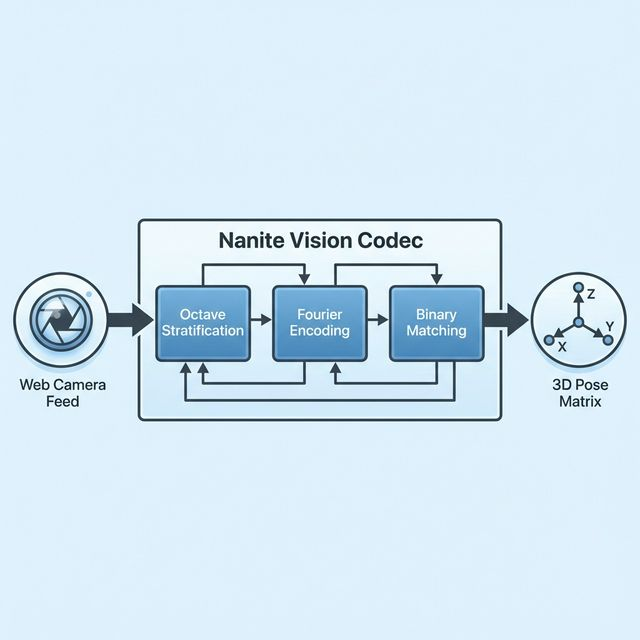
\includegraphics[width=\columnwidth]{figures/fig1_architecture.png}}
\caption{System Architecture of TapTapp AR V11, demonstrating the pure JavaScript pipeline and the integration of the Nanite Vision Codec.}
\label{fig1}
\end{figure}

\subsubsection{Step B: Implementation of the Vision Codec}
The feature extraction algorithms were implemented to output 4-bit packed tracking data and 64-bit LSH fingerprints. This step focused on maximizing the information density per byte of the output file.

\begin{figure}[htbp]
\centerline{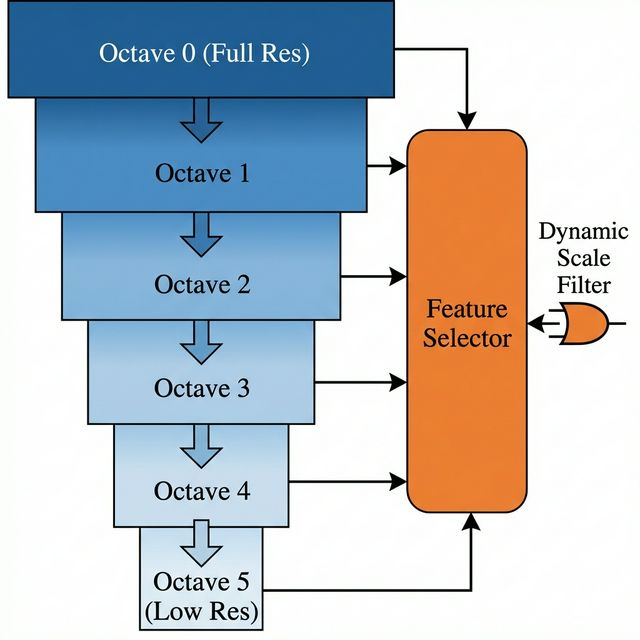
\includegraphics[width=\columnwidth]{figures/fig2_feature_stack.png}}
\caption{Nanite Feature Extraction Pipeline, illustrating the multi-octave stratification and dynamic scale filtering mechanism.}
\label{fig2}
\end{figure}

\begin{figure}[htbp]
\centerline{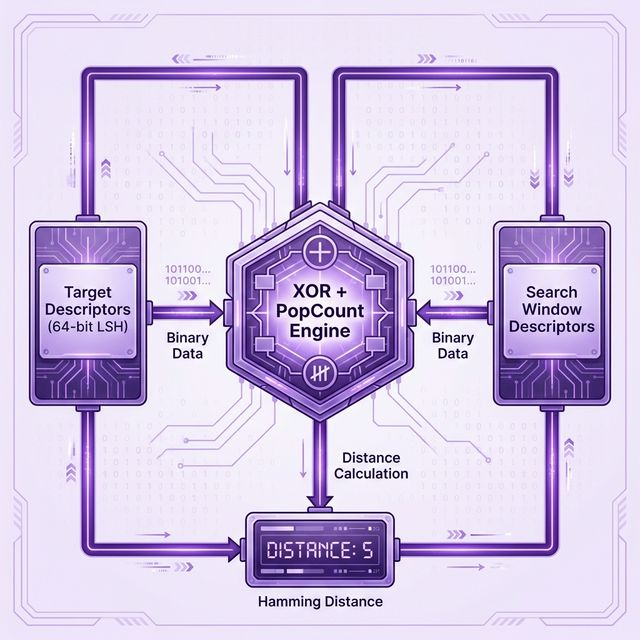
\includegraphics[width=\columnwidth]{figures/fig3_matching_engine.png}}
\caption{Binary Matching Engine Logic, detailing the XOR and PopCount operations used for high-speed descriptor matching.}
\label{fig3}
\end{figure}

\subsubsection{Step C: Integration of the JIT Compiler}
A Just-In-Time (JIT) compilation module was developed to process images directly in the browser. This module handles the conversion of standard images into the proprietary \texttt{.taar} format on the fly.

\subsubsection{Step D: Comparative Benchmarking}
The final phase involved the systematic collection of performance data. A simulated environment was set up to run 45 iterations of compilation and tracking for both the control and experimental groups. Metrics such as compilation time (in seconds), output file size (in KB), and detection stability were recorded for statistical analysis.

\begin{figure}[htbp]
\centerline{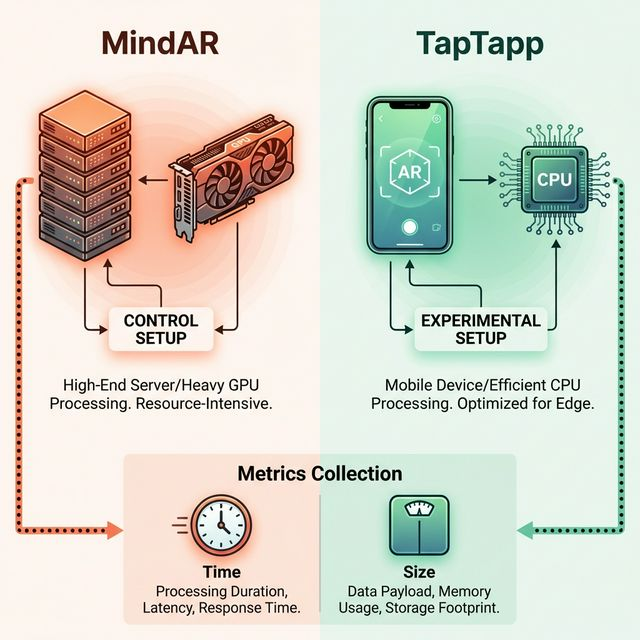
\includegraphics[width=\columnwidth]{figures/fig4_experiment_setup.png}}
\caption{Experimental Setup Comparison: MindAR (Control) vs. TapTapp AR (Experimental), highlighting the hardware and metric collection focus.}
\label{fig4}
\end{figure}
